\section{Метод Ньютона-Рафсона}

\textbf{Алгоритм метода}:
$$ x^{k + 1} = x^{k} - t_{k}H^{-1}(x^{k})\nabla f(x^{k}) $$

$d^{k} = -H^{-1}(x^{k})$ --- направление спуска.

$t_{k}$ --- шаг выбирается из условия убывания функции в точках последовательности: $f(x^{k + 1}) < f(x^{k})$.

Основной критерий окончания метода: $||\nabla f(x^{k})|| < \varepsilon$.

Начальные параметры метода: $x^{0}, \varepsilon$.

Изменяемые параметры метода: величина шага $t_{k}$.

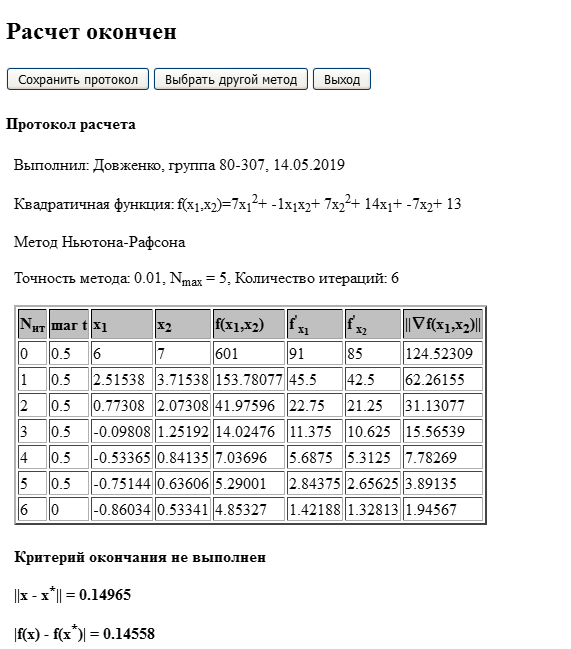
\includegraphics[width=0.8\linewidth]{om_hw_01/images/3.PNG}\\
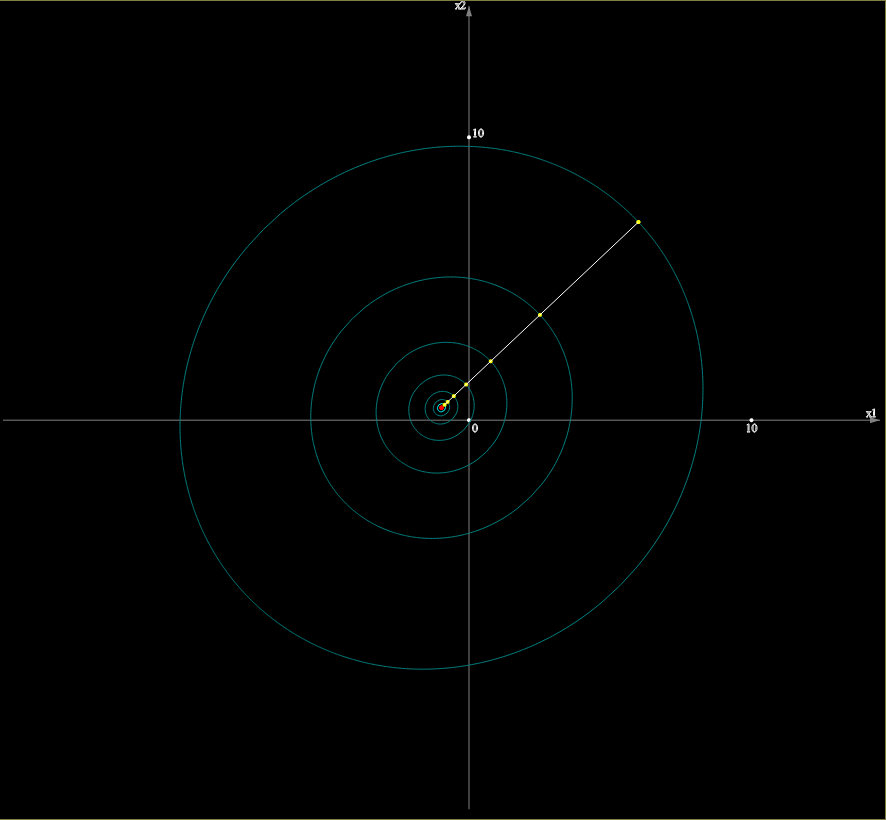
\includegraphics[width=0.8\linewidth]{om_hw_01/images/3_2.PNG}\\

\textbf{Последняя итерация}:\\
$x^{5} = x^{4} - t_{4}H^{-1}|x^{4}| \nabla f(x^{4})$\\
$x^{4} = 
\begin{pmatrix}
  -0.53365\\
  0.84135
\end{pmatrix}
$\\

$t_{4} = 0.5$\\
$
H^{-1}(x^{4}) = 
\begin{pmatrix}
  0.0717 & 0.0051\\
  0.0051 & 0.0717
\end{pmatrix}
$\\

$
\nabla f(x^{4}) = 
\begin{pmatrix}
  14x_{1} - x_{2} + 14\\
  14x_{2} - x_{1} - 7
\end{pmatrix}
=
\begin{pmatrix}
  5.68755\\
  5.31255
\end{pmatrix}
$\\

$
x^{5} = 
\begin{pmatrix}
  -0.53365\\
  0.84135
\end{pmatrix}
-
0.5
\begin{pmatrix}
  0.43488\\
  0.409906
\end{pmatrix}
=
\begin{pmatrix}
  -0.75109\\
  0.636397
\end{pmatrix}
$\\

$||\nabla f(x^{5})|| \approx 2.2977 > \varepsilon$

\pagebreak